\subsection{Design (Machac)}
Das Folgende wurde von Phillip Machac geschreiben. Er war als eine Art externer Mitarbeiter für das Design der Seite verantwortlich. Die Implementierung wurde allerdings vom SIS-Team durchgeführt.
\subsubsection{Enstehung}
Die grundsätzliche Idee war es, ein Design zu schaffen welches, im Gegensatz zu den meisten anderen Dingen unserer Anstalt, einladend und angenehm zu betrachten ist. Des Weiteren sollte der Betrachter nicht in Gefahr kommen, bei Ansicht der Supplierungen Augenkrebs oder ähnlich tragische Krankeiten zu erleiden *räusper* Wirtschaft *räusper* :D. Dementsprechend wurde ein unauffälliger Hintergrund mit warmen Farben gewählt, in diesem Fall Brauntöne. Als angenehm empfand ein Großteil der befragten Personen einen Holzhintergrund, von Verfechtern oftmals nur „Wohnzimmerboden“ genannt.\\
Da zum Zeitpunkt des Entwurfes gerade eine hitzige Diskussion bezüglich des Namens im Gange war (HTL Peter Anich, HTLinn oder einfach HTL Anichstraße) wurde das Design daraufhin ausgelegt, egal wie diese Diskussion auch enden sollte, autonom und für jegliche Änderungen gerüstet zu sein.\\
Das Logo der HTL mag ein toller Einfall gewesen sein, bezogen auf die Form und die Umsetzung der 4 Abteilungsfarben im Logo, zur Einpflegung in ein Design stellt es allerdings aufgrund der vielen unterschiedlichen Farben eine mittlere Katastrophe dar. Deswegen wurde entschieden das Logo einfarbig (Schwarz mit Transparenz) mit durchsichtigen Konturrändern, zur besseren Unterscheidung der Flächen innerhalb des Logos, umzubauen. Durch diesen Effekt wirkt das Logo fast wie \enquote{auf dem Holz eingebrannt}.\\
\enquote{Simplicity} ist eine weitere Eigenschaft, die das Design auszeichnen sollte, weshalb das gesamte Layout darauf ausgelegt ist, mit zwei, maximal aber 3 Farben auszukommen. Zulässige Schriftfarben sind nur Schwarz (ggf. mit Transparenz) und Weiß, sämtliche Grafiken sind Schwarz mit einer Opacity (Transparenz) und nur Transparent (also Hintergrund kommt durch).\\
Da zu  einem schlichten Design auch die verwendete Schriftart eine beträchtliche Rolle spielt, wurde von uns, die unserer Ansicht nach sehr schlichte Font \enquote{Century Gothic} verwendet. Diese zieht sich ebenfalls durch das ganze System, vom Webinterface über die App bis zu den Monitoren. Lediglich für den Text im Banner wurde ein auffälligerer, etwas freakig wirkender Schriftzug verwendet (Abduction2002), welcher dem Benutzer mitteilt, wo er sich befindet bzw. was er gerade sieht, z.B. SIS.Web Access oder auf den Monitoren z.B. SIS.Supplierungen oder SIS.News.\\
Diese Elemente (Header, Hintergrund und Logo) ziehen sich sowohl im Webinterface als auch auf den Monitoren wie ein roter Faden durch das System.\\
\subsubsection{Webinterface}
\label{sec:content_draft_design_web}
Das Webinterface sollte einen \enquote{WOW – Das ist aber cool}-Effekt erzeugen. Die einzelnen Menüpunkte sollten logisch angeordnet sein und sich gut in das Gesamtbild mit modifiziertem HTL Bild und Hintergrund einbinden. Deshalb wurde die Idee geboren, das Logo in der Mitte als zentralen Ausgangspunkt für die Menüführung zu verwenden. Die Buttons wachsen als Parallelogramme aus den vier Flächen des Logos, jeweils maximal zwei. Wird also die Maximalanzahl von acht Buttons erreicht, wirkt das Gesamtpaket einem Raumschiff ähnlich – sehr cool ;-).\\
Um die Menüführung für den Benutzer sinnvoll und übersichtlich zu gestalten und trotzdem die Maximalanzahl an Buttons pro Seite nicht zu überschreiten wurde die Menüführung in drei Teile aufgeteilt.\\
Die erste Seite stellt Informationen für den User da, unabhängig davon, ob dieser selbst noch Administrative Funktionen erfüllt oder nicht. Es werden seine persönlichen Supplierungen, sein persönlicher Stundenplan und die Newsansicht zur Verfügung gestellt. Der Button rechts unten stellt jeweils den Schritt zum nächsten Menü dar. Auf der zweiten Seite finden sich Administrative Möglichkeiten wieder, welche für den täglichen Gebrauch nötig sind. Hier sind also Punkte zur Eingabe der Supplierpläne und der fehlenden Lehrer, der News und das Management der Monitore. Auffällig ist hier, dass der Versuch unternommen wurde, zusammengehörige Punkte auch so anzuordnen (Menüübergreifend). So findet sich rechts oben auf der ersten Seite (SIS.Web Access) die Anzeige der Supplierungen, auf der zweiten Seite (SIS.Inputs) die Eingabe der fehlenden Lehrer und der Supplierungen wieder. Ebenso links unten die News zur Anzeige auf der ersten, die Eingabe selbiger auf der zweiten Seite. Somit ist das Menü etwas intuitiver gestaltet, als wenn die Anordnung anders wäre.\\
Da die zahlreichen Administrationsmöglichkeiten eine Seite mit acht Buttons sprengen würde, wurden eher selten genutzte Funktionen wie das Ändern der Stunden oder die Eingabe neuer Lehrer oder Stundenpläne auf ein drittes Menü ausgelagert (SIS.Administration), welches wiederum über den Button rechts unten erreicht werden kann.\\
\begin{figure}[H]
\centering
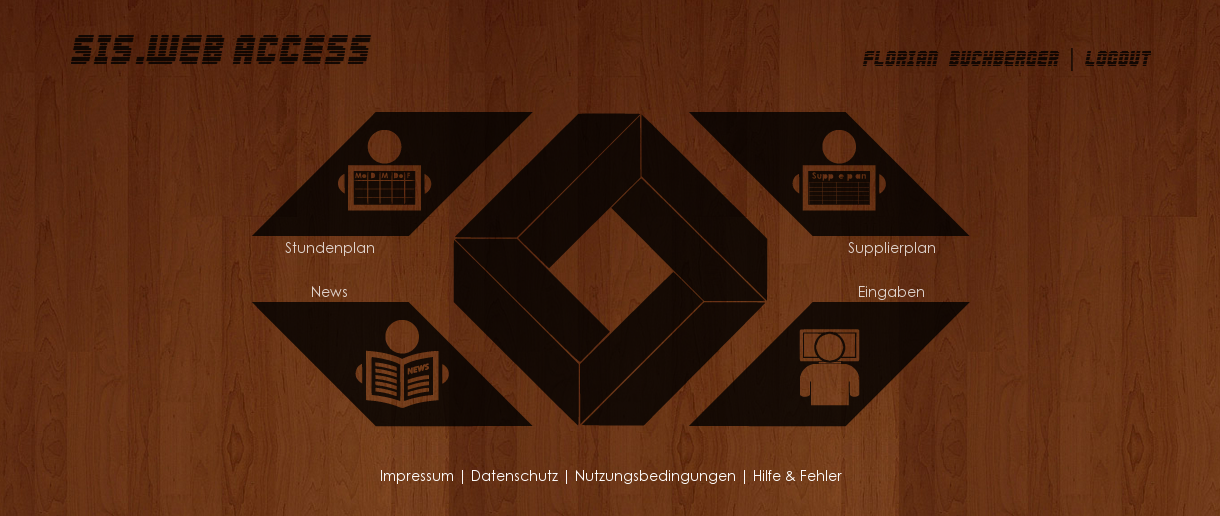
\includegraphics[keepaspectratio=true, width=14cm]{images/screenshots/web-access_nohover.png}
\caption{SIS.Web Access}
\label{fig:content_draft_design_webaccess}
\end{figure}
\begin{figure}[H]
\centering
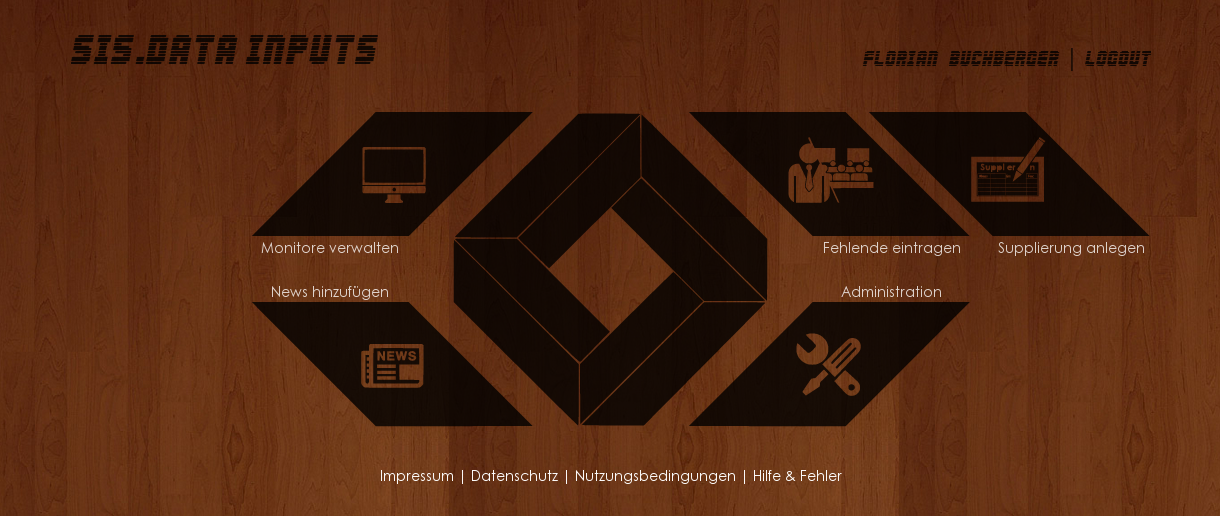
\includegraphics[keepaspectratio=true, width=14cm]{images/screenshots/data-inputs_nohover.png}
\caption{SIS.Data Inputs}
\label{fig:content_draft_design_datainputs}
\end{figure}
\begin{figure}[H]
\centering
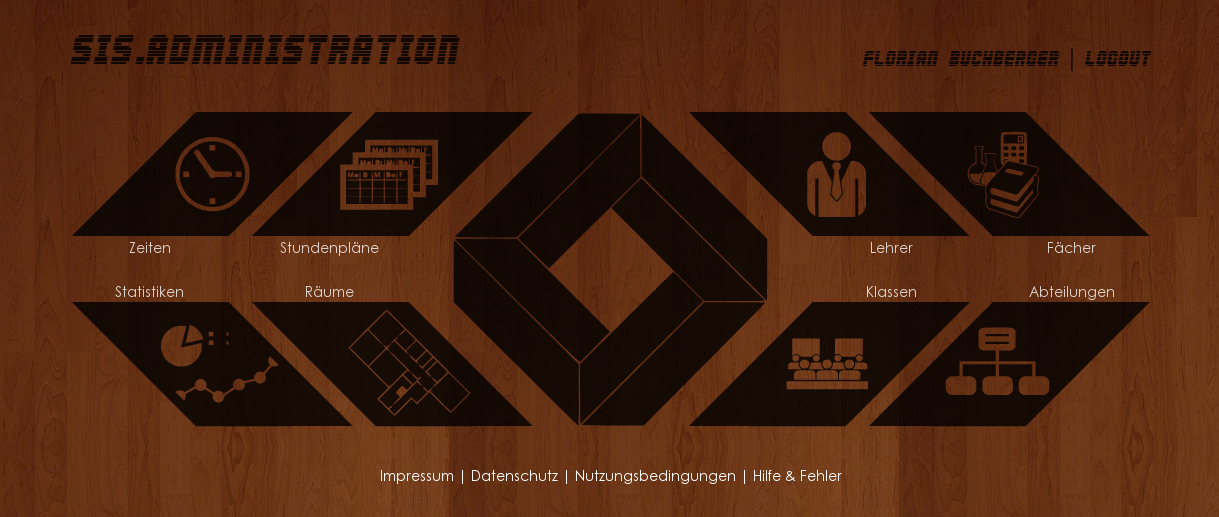
\includegraphics[keepaspectratio=true, width=14cm]{images/screenshots/administration_nohover.png}
\caption{SIS.Administration}
\label{fig:content_draft_design_administration}
\end{figure}
Mit Klick auf das Logo in der Mitte gelangt man jeweils zum vorhergehenden Menü zurück.\\
Die Buttons enthalten jeweils eine Grafik, welche den Punkt für den dieser Button steht, bestmöglich repräsentieren sollte. Ein Hoover Effekt bewirkt eine Änderung der Buttonfarbe (Schwarz auf Weiß) und weist den User daraufhin, welchen Button er aktuell gewählt hat. Dieser Effekt benötigt allerdings SVG Grafiken anstatt Beispielsweise png's, was die ganze Sache etwas kompliziert macht, dafür jedoch auch weniger Traffic – svg Grafiken sind kleiner – verursacht.\\
Da der Inhalt, welchen man erreichen soll nachdem ein Button geklickt wurde, seine Zusammengehörigkeit mit der eigentlichen Navigation/Menü nicht verlieren sollte wurde beschlossen, dass der neue Inhalt im Zuge einer Animation erscheint. Wird also ein Button angeklickt, wird der Monitor optisch quasi horizontal geteilt und auseinander geschoben. Im sich nun öffnenden Teil des Bildschirmes erscheint nun ein leicht dunklerer Hintergrund (ebenfalls Brauntöne), auf dem sich nach Beenden der Animation der Inhalt aufbaut. Um den Übergang zwischen den beiden Hintergründen sanfter zu gestalten, wurde eine weiße Linie dazwischen gezogen. Will man wieder in das Menü, kann nun entweder außerhalb des dunklen Hintergrundes auf den Bildschirm geklickt werden, oder der Exit Button verwendet werden. Die Animation wird daraufhin entgegengesetzt ausgeführt und man ist wieder im ursprünglichen Menü.\\
All diese Features sind allerdings nur dann möglich, wenn Javascript aktiviert ist. Sollte das am Client PC nicht der Fall sein, wird eine Javascript-freie Seite geladen, ohne Animationen im Menü und lediglich mit der Möglichkeit, durch Anklicken des zugehörigen Buttontextes, den betreffenden Inhalt zu laden. Dieser erscheint in einem Vollbild und kann nur mit dem Exit Button wieder verlassen werden. Auf mobilen Geräten (iPhone, Android Devices usw.) wird zudem NUR die Seite ohne JS geladen, auch wenn das Device JS unterstützen würde.
\subsubsection{Monitordesign}
Die wichtigsten Inhalte, welche am Monitor angezeigt werden sind News, Supplierungen und Raumpläne. Die News werden mit weißer Schriftart in einem Schwarz transparenten Fenster mit abgerundeten Ecken angezeigt. Die Supplierungen in einer Tabelle, welche wiederum weiße Schrift auf schwarz transparentem Hintergrund ist, wobei die erste Zeile inverse Farben verwendet. Besonderheiten bei dieser Tabelle ist die Sortierung, welche nach Klassen erfolgt (vereinfacht das Lesen für die Schüler) sowie der Verzicht auf Vertikale Spaltenabtrennungen. Dies ermöglicht ein angenehmeres Lesen der Supplierungen. Die Raumbelegungspläne haben dieselbe Farbabstimmung wie der Supplierplan. Jede Zelle zeigt die drei Inhalte Klasse, Lehrer und Fach an, wobei die Klasse größer in der ersten Zeile und das Fach mit dem Lehrer in der nächsten Zeile in kleinerer Schriftart abgebildet sind.